\documentclass{report}

\usepackage{textcomp}
\usepackage{graphicx}
\usepackage{fancyhdr}
\usepackage{subcaption}
\usepackage{multicol}
\usepackage{outlines}
%===================================
\newcommand{\classinfo}{{\bf Router On \\ A Stick}\\{\it CIT 167}\\{Chaz Davis}}
\newcommand{\semester}{BCTC \\ Spring 2020}
%===================================
\newcommand{\mysection}[1]{\section*{#1}}
\newcommand{\mysubsection}[2]{\textbf{\romannumeral #1) #2}}
%===================================
\setlength{\headheight}{15.2pt}
\pagestyle{fancy}
\fancyhf{}
\lhead{ \fancyplain{}{Chaz Davis} }
\rhead{ \fancyplain{}{\today} }
\cfoot{ \fancyplain{}{\thepage} }
\renewcommand{\headrulewidth}{0.5pt}
\renewcommand{\footrulewidth}{0pt}

%===================================
\title{\classinfo}
\author{\semester}
\date{\today}

%===================================

\begin{document}

\maketitle

%===================================
\mysection{\textbf{Part 1: Configuring and verifying the Network}}

I First set up the network according to the diagram.
I then, Configured the Ip address, subnet masks, and default gateways for the
PCs according the chart.
I then, configured the Switch and router according to the handout.

Successfully able to ping PC3 from PC1.


\begin{figure}[!hbt]\centering
\subfloat[Pinging PC3 from
PC1]{\label{success15ping}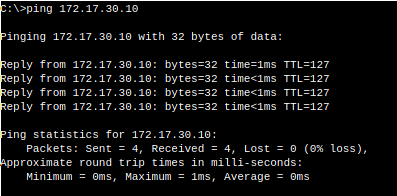
\includegraphics[width=.45\linewidth]{Figures/2020-03-08-191601_397x196_scrot.png}}\par
\subfloat[Successful Network
COnfiguration]{\label{success15net}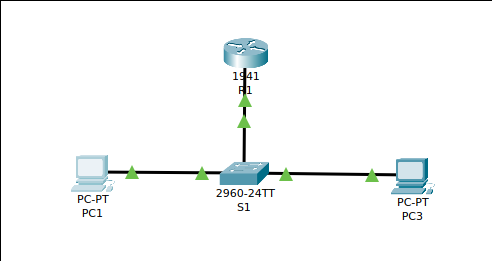
\includegraphics[width=.45\linewidth]{Figures/2020-03-08-191611_492x261_scrot.png}}\par
\caption{Successful network setup}
\label{success15}
\end{figure}








%===================================

\end{document}
